\documentclass[8pt]{beamer}
\usetheme{default} % Very simple theme
\usecolortheme{dove} % Minimalist grayscale colors
\setbeamertemplate{navigation symbols}{} % Remove navigation bar

% Define brand-like colors
\definecolor{myblue}{RGB}{0, 102, 204}    % Blue for standard blocks
\definecolor{mygreen}{RGB}{0, 153, 0}     % Green for example blocks
\definecolor{myred}{RGB}{204, 0, 0}       % Red for alert blocks
\definecolor{myorange}{RGB}{255, 128, 0} % For \emph

% Accent color for titles, bullets, etc.
\setbeamercolor{structure}{fg=myblue}

% Block colors
\setbeamercolor{block title}{bg=myblue, fg=white}
\setbeamercolor{block body}{bg=blue!5, fg=black}

\setbeamercolor{exampleblock title}{bg=mygreen, fg=white}
\setbeamercolor{exampleblock body}{bg=green!5, fg=black}

\setbeamercolor{alertblock title}{bg=myred, fg=white}
\setbeamercolor{alertblock body}{bg=red!5, fg=black}
\setbeamercolor{alerted text}{fg=myred}

% Optional: color for \example text
\setbeamercolor{example text}{fg=mygreen}

% Custom emph (orange text instead of italic)
\let\oldemph\emph
\renewcommand{\emph}[1]{\textcolor{myorange}{#1}}


\usepackage{graphicx} % Package for images
\usepackage{amsmath} % Package for images
\graphicspath{{figs/}} % Path to your figures directory
\usepackage{array}  % For better column spacing
\usepackage{caption} % Required for \captionof

% Title Information
\title{STOCHASTIC METHODS IN WATER RESOURCES}
\vspace{25pt}
\subtitle{Unit 2: Hydrological statistics and extremes \\ Lecture 6: Probability distributions of extremes, distribution selection}
\author{Luis Alejandro Morales, Ph.D.}
\institute{Universidad Nacional de Colombia \\ Department of Civil and Agriculture Engineering} %// }
%\date{\today}

\begin{document}

% Title Slide
\begin{frame}
    \titlepage
\end{frame}

%-------
% From Diaz-granados
\section{Probability distributions of extremes}
\subsection{Gumbel distribution}
\begin{frame}{Gumbel distribution}
    The \alert{Gumbel distribution} is equivalent to the to asymptotic  distribution type I and result from a basic \emph{exponential distribution}. The \emph{Gumbel distribution} has two parameters: the \emph{scale parameter} $\alpha$ and the \emph{position parameter} $b$, and is given for \emph{maximum values} represented by $X$, where:
    \[
        f_X (x) = \frac{1}{\alpha} e^{\left[ -\frac{x-b}{\alpha} -e^{\left( - \frac{x-b}{\alpha} \right) }\right]}, \text{ for } -\infty < x < \infty
    \]
    The \emph{cdf} is:
\[
    F_X (x) = e^{\left[-e^{\left( -\frac{x-b}{\alpha} \right)} \right]}
\]
and $\mu_X = b + 0.5772 \alpha$ and $\sigma_X^2 = \frac{\pi^2 \alpha^2}{6}$ and the asymmetry coefficient $\gamma_1 = 1.1396$. The \emph{quantile} of this distribution is:
\[
x(F) = b - \alpha \ln(-\ln F)
\]
where $x(F)$ is the value of $X$ for which the \emph{cdf} value is $F$. This equation is equivalent to:
\[
    x_T = b - \alpha \ln \left[ -\ln \left( 1- \frac{1}{T} \right) \right]
\]
where $T$ is the \emph{return period} and $x_T$  is the magnitude of the extreme event associated to this. 
\end{frame}

\begin{frame}{Gumbel distribution}
    The parameter estimation in the \emph{Gumbel distribution} can be performed using different methods such as the Moments and the Maximum-Likelihood. The \emph{frequency factor} $K_T$ for this distribution when $n\rightarrow \infty$, converge asyntotically to:
    \[
        K_T = - \frac{\sqrt{6}}{\pi} \left[ 0.5772 + \ln \left( \ln \left( 1-\frac{1}{T} \right) \right) \right]
    \]
    On the other hand, for a value of the annual series, the \emph{frequency factor} as a function of the size series, can be estimated as:
    \[
        K_m = \frac{y_m - \bar{y}}{s_y}
    \]
    where:
\[
    y_m  = -\ln \left[ -\ln \left( \frac{n+1-m}{n+1} \right) \right]
\]
Note that the data are sorted in descending order; from the largest ($m=1$) to the smallest ($m=n$). $\bar{y} = \frac{1}{n} \sum_{m=1}^n y_m$ and $s_y^2 = \frac{1}{n} \sum_{m=1}^n (y_m - \bar{y})^2$.
For a \emph{return period} $T$, the \emph{frequency factor} is:
\[
    K_T = \frac{y_T - \bar{y}}{s_y}
\]
where $y_T = -\ln \left[ -\ln \left( 1- \frac{1}{T} \right) \right]$. Comparing the two equations to compute $K_T$ the later equations provide larger results of $K_T$ than the former one. This value is progressively larger as much as $n$ decrease. This means that the shorter the series the larger the values of $x_T$. 
\end{frame}

\begin{frame}{Gumbel distribution}
    Estimation of the \emph{standard deviation $s_T$} using different methods:
    \begin{itemize}
        \item \emph{Method of Moments}
            \[
                s_T^2 = \frac{s_X^2}{n} \left[ 1 + K_T \gamma_1 + \frac{K_T^2}{4} (\gamma_2 - 1) \right]
            \]
            where $\gamma_1 = 1.1396$ and $\gamma_2 = 5.4002$
        \item \emph{Method of Maximum-Likelihood}
            \[
            s_T^2 = \frac{\hat{\alpha}^2}{n} \left[ 1 + \frac{6}{\pi^2} (1-0.5772 + y_T )^2 \right]
        \]

        \item \emph{Method of MPP}
            \[
            s_T^2 = \frac{\hat{\alpha}^2}{n} \left[ 1.1128 + 0.4574 y_T + 0.8046 y_T^2 \right]
        \]
    \end{itemize}
\end{frame}

\begin{frame}{Gumbel distribution}
    So far, we have analysed annual series of \emph{maximum values} using the \emph{Gumbel distribution}. However, this distribution can be used to analyzed \emph{minimum values} $Z$ so the \emph{pdf} is: 
    \[
        f_Z (z) = \frac{1}{\alpha} e^{\left[ \frac{z-b}{\alpha} -e^{\left( \frac{z-b}{\alpha} \right) }\right]}, \text{ for } -\infty < z < \infty
    \]
    and the \emph{cdf} is: 
\[
    F_Z (z) = 1- e^{\left[-e^{\left( \frac{x-b}{\alpha} \right)} \right]}
\]
The $\mu_Z = b - 0.5772 \alpha$, $\sigma_Z^2 = \frac{\pi^2 \alpha^2}{6}$ and the asymmetry coefficient is $\gamma_1 = -1.1396$. The \emph{quantile} is:
\[
z(F) = b + \alpha \ln(-\ln (1-F))
\]
where $z(F)$ is the value of $Z$ for which the \emph{cdf} value is $F$. This equation is equivalent to:
\[
    z_T = b + \alpha \ln \left[ -\ln \left( 1- \frac{1}{T} \right) \right]
\]
Similarly, the parameter of the distribution can be estimated using different methods.
\end{frame}


\begin{frame}{Gumbel distribution}
When $n\rightarrow \infty$ asymptotically, the \emph{frequency factor $K_T$} converge to :
    \[
        K_T =  \frac{\sqrt{6}}{\pi} \left[ 0.5772 + \ln \left( -\ln \left( 1-\frac{1}{T} \right) \right) \right]
    \]
    On the other hand, for a value of the annual series, the \emph{frequency factor} as a function of the size series, can be estimated as:
    \[
        K_m = \frac{\bar{y} - y_m }{s_y}
    \]
    where:
\[
    y_m  = \ln \left[ -\ln \left( \frac{m}{n+1} \right) \right]
\]
Note that the data are sorted in ascending order; from the smallest ($m=1$) to the largest ($m=n$). $\bar{y} = \frac{1}{n} \sum_{m=1}^n y_m$ and $s_y^2 = \frac{1}{n} \sum_{m=1}^n (y_m - \bar{y})^2$.

For a \emph{return period} $T$, the \emph{frequency factor} is:
\[
    K_T = \frac{\bar{y} - y_T}{s_y}
\]
where $y_T = -\ln \left[ -\ln \left(- \frac{1}{T} \right) \right]$. 
\end{frame}

\begin{frame}{Pearson type III and Log-Pearson type III distributions}
    The \emph{pdf} of the \alert{Pearson type III distribution} is:
    \[
        f_X (x) = \frac{1}{a \Gamma (b)} \left( \frac{x-c}{a} \right)^{b-1} e^{\left[ - \left( \frac{x-c}{a} \right) \right]}
        \]
        where the parameters $a$, $b$ and $c$ are the scale, the shape and the position, respectively. Note that $b>0$ and that $c < x < \infty$. If $c = 0$, the \emph{pdf} is reduced to the \emph{Gamma distribution}. Despite $a$ can be either positive or negative, if $a<0$ the \emph{pdf} is bounded above, this means that $x < c$ and it is not suitable to analyse maximum extreme events. Using the \emph{methods of Moments}:
        \begin{itemize}
            \item \emph{Mean}
                \[
                    \mu_X = c + ba
                \]

            \item \emph{Variance}
                \[
                    \sigma_X^2 = ba^2
                \]
            \item \emph{Asymmetry coefficient}
                \[
                    \gamma_1 = sgn(a) \frac{2}{\sqrt{b}}
                \]
                where $sgn$ is the sign function.
        \end{itemize}
        Sometimes, the annual series are transformed using the logarithm function and the data is fitted to the \emph{Pearson type III distribution}, which is equivalent to the \alert{Log-Pearson type III distribution}. This distribution is commonly used to analyse maximum streamflows and requires that $b>1$ and $a>0$. The equations to estimate the frequency factor are given in textbook tables. 

\end{frame}

\begin{frame}{Weibull distribution}
    The \alert{Weibull distribution} is equivalent to the asymptotic type III distribution, and is popular to the analysis of annual series of minimum values $Z$. The \emph{pdf} is defined as:
    \[
        f_Z (z) = \left( \frac{\kappa}{\alpha} \right) \left( \frac{z-b}{\alpha} \right)^{\kappa -1} e^{\left[ - \left( \frac{z-b}{\alpha} \right)^\kappa \right]}
    \]
    where $z \geq b$, $\alpha > b $ and $\kappa > 0$. The \emph{cdf} is:
    \[
        F_Z (z) = 1- e^{\left[ - \left( \frac{z-b}{\alpha} \right)^\kappa \right]}
    \]
    Some expressions are:
        \begin{itemize}
            \item \emph{Mean}
                \[
                    \mu_Z = b + \alpha \Gamma \left(1 + \frac{1}{\kappa} \right)
                \]

            \item \emph{Variance}
                \[
                    \sigma_Z^2 = \alpha^2 \left[ \Gamma \left( 1 + \frac{2}{\kappa} \right) - \Gamma^2 \left( 1 + \frac{1}{\kappa} \right) \right]
                \]
            \item \emph{Asymmetry coefficient}
                \[
                    \gamma_1 = \frac{\Gamma \left( 1 + \frac{3}{\kappa} \right) - 3\Gamma \left( 1 + \frac{1}{\kappa} \right)\Gamma \left( 1 + \frac{2}{\kappa} \right) + 2\Gamma^3 \left( 1 + \frac{1}{\kappa} \right) }{\left[\Gamma \left( 1 + \frac{2}{\kappa} \right) - \Gamma^2 \left( 1 + \frac{1}{\kappa} \right) \right]^{1.5}}
                \]
                where $\Gamma(.)$ is the \emph{Gamma function}.
        \end{itemize}
         The inverse of the \emph{ Weibull cdf} is:
         \[
             z(F) = b + \alpha \left[ -\ln \left(1-F \right) \right]^{1/\kappa}
         \]
         Note that when $\kappa = 1$ this distribution becomes the \emph{exponential distributio}. Other properties of the \emph{Weibull distribution} are given in textbooks tables. 

\end{frame}

\begin{frame}{Fr\'echet distribution}
    The \alert{Fr\'echet distribution} is equivalent to the asymptotic type II distribution. The \emph{pdf} is defined as:
                \vspace{-5pt}
    \[
        f_X (x) = \frac{\theta}{a} \left( \frac{a}{\theta} \right)^{\theta +1} e^{\left[ - \left(\frac{a}{x}\right)^{\theta} \right]}
    \]
    where $x>0$, and the scale and  shape parameters are  $a>0$ and $\theta >0$, respectively. The \emph{cdf} is:
    \[
        F_X (x) = e^{\left[ - \left( \frac{a}{x} \right)^{\theta} \right]}
        \]
    Some expressions are:
        \begin{itemize}
            \item \emph{Mean}
                \vspace{-5pt}
                \[
                    \mu_X = a \Gamma \left( 1 - \frac{1}{\theta} \right)
                \]
                valid when $\theta > 1$

            \item \emph{Variance}
                \vspace{-5pt}
                \[
                    \sigma_X^2 = a^2 \left[ \Gamma \left(1- \frac{2}{\theta} \right) - \Gamma^2 \left( 1- \frac{1}{\theta} \right) \right] 
                \]

                \[
                    V_X = \left[ \frac{\Gamma (1-2/\theta)}{\Gamma^2 (1-1/\theta)} -1\right]^{0.5} 
                \]
                where the functions for $\sigma_X^2$ and $V_X$  are valid for $\theta > 2$.         
        \end{itemize}
The quantile for the \emph{Fr\'echet pdf} is given:
                \[
                    x(F) = a (-\ln F )^{-\theta}
                \]
                Regarding  to the exponential positive shape for $\theta > 0$, $x(F)$ increases faster than the \emph{Gumbel distribution}  when $F$ increase. This means that \emph{Fr\'echet distribution} produces a frequency curve of larger magnitudes. These two distributions are related through the \emph{logarithm transform}, because when $X$ follow a \emph{Fr\'echet pdf} with parameters $a$ and $\theta$, $Y = \ln (X)$ follow a \emph{Gumbel pdf} with parameters $\alpha = 1/\theta$ and $b = \ln (a) $. Other properties of the \emph{Fr\'echet distribution} are given in textbooks tables. 

\end{frame}

\begin{frame}{GEV distribution}
    The \alert{Generalized Extreme Value (GEV) distribution} is used for extreme maximum values, usually meteoroligical data. The \emph{pdf} is:
    \[
        f_X (x) = \frac{1}{a} \left[ 1- \frac{b}{a} (x-c) \right]^{(1-b)/b} e^{ -\left[ 1- \frac{b}{a} (x-c) \right]^{1/b}}    
    \]
    and the \emph{cdf} is:
    \[
        F_X (x) = e^{ -\left[ 1- \frac{b}{a} (x-c) \right]^{1/b}}
    \]

    where $a>0$, $b$ and $c$ are the parameters of scale, shape and position, respectively. If $b>0$ the distribution is bounded above representing a type III distribution which is useful for the analysis of extreme mimimum events. In contrast, if $b<0$ the distribution is bounded below equivalent to a type II distribution suitable for extreme maximum events. If $b=0$, the \emph{GEV distribution} is transformed to a \emph{Gumbel distribution}. 

    The fist two moments are:
        \begin{itemize}
            \item \emph{Mean}
                \vspace{-5pt}
                \[
                    \mu_X = c + \frac{a}{b} [1- \Gamma (1+b) ] 
                \]

            \item \emph{Variance}
                \vspace{-5pt}
                \[
                    \sigma_X^2 = \frac{a^2}{b^2} [\Gamma (1 + 2b) - \Gamma^2 (1+b) ] 
                \]
                where $\Gamma(r)$ is the \emph{Gamma function} evaluated in $r$. Note that while the equation for $\mu_X$ is valid for $b > -1$, the equation for $\sigma_X^2$ is valid for $b > -0.5$. A quantile is computed as:
                \[
                    x(F) = c + \frac{a}{b} \left[ 1- (-\ln F)^b \right] 
                \]

        \end{itemize}
Other properties of the \emph{GEV distribution} are given in textbooks tables. 

\end{frame}

\begin{frame}{Pareto distribution}
    The \alert{Pareto distribution} is commonly used to analysed variables with long, straight tails. This distribution was initially implemented to analysed the wealth distribution in society where a low percentage concentrate the largest wealth. The   \emph{pdf} \emph{classic Pareto distribution} or \emph{Pareto I distribution} is:
    \[
        f_x (x) = a_I c_I^{a_I} x^{a_I -1}
    \]
    where $x > c_I$ and $a_I > 0$. $c_I$ and $a_I$ are the position and shape parameters, respectively. The \emph{cdf} is:
\[
    F_X (x) = 1-\left(\frac{c_I}{x} \right)^{a_I}
\]
    The fist two moments are:
        \begin{itemize}
            \item \emph{Mean}
                \[
                    \mu_X = \frac{c_I a_I}{a_I -1}
                \]
                Note that this is valid when $a_I > 1$, and $\infty$ on the contrary. 

            \item \emph{Variance}
                \[
                    \sigma_X^2 = \left( \frac{cI}{a_I - 1} \right)^2 \frac{a_I}{a_I -2}
                \]
                when $a_I > 2$. If $1 < a_I \leq 2$, $\sigma_X^2 = \infty$, and not exist when $a_I \leq 1$.

        \end{itemize}

\end{frame}

\begin{frame}{Pareto distribution}
    The \emph{Pareto I distribution} is embeded in a more general \emph{Pareto II distribution}. The \emph{pdf} of this distribution is:
 \[
f_X (x) =
\begin{cases}
    \frac{1}{b} \left( 1- a\frac{x}{b} \right)^{\frac{1}{a} -1} & \text{for } a \neq 0  \\
    \frac{1}{b} e^{\left( -\frac{x}{b} \right)} & \text{for } a = 0 
\end{cases}
\]
The \emph{cdf} is:
 \[
F_X (x) =
\begin{cases}
    1- \left( 1- a\frac{x}{b} \right)^{\frac{1}{a}} & \text{for } a \neq 0  \\
    1- e^{\left( -\frac{x}{b} \right)} & \text{for } a = 0 
\end{cases}
\]

where $b$ is the scale parameter. 
Including a third parameter $c$, the position parameter, the \emph{pdf} of the \emph{Pareto III distribution} is:
 \[
f_X (x) =
\begin{cases}
    \frac{1}{b} \left( 1- a\frac{x-c}{b} \right)^{\frac{1}{a} -1} & \text{for } a \neq 0  \\
    \frac{1}{b} e^{\left( -\frac{x-c}{b} \right)} & \text{for } a = 0 
\end{cases}
\]
The \emph{cdf} is:
 \[
F_X (x) =
\begin{cases}
    1- \left( 1- a\frac{x-c}{b} \right)^{\frac{1}{a}} & \text{for } a \neq 0  \\
    1- e^{\left( -\frac{x-c}{b} \right)} & \text{for } a = 0 
\end{cases}
\]
Note that when $c=0$, the \emph{Pareto III distribution} becomes the \emph{Pareto II distribution}. Also, when $a< 0$ and $c=0$ becomes the \emph{Pareto I distribution} with $a_I = 1/a$ and $c_I = -b/a $. 

\end{frame}

\begin{frame}{Frequency curves for minimum events}
    \begin{itemize}
        \item The commonly implemented probability distributions to analysed annual series of minimum events are: \emph{Weibull}, \emph{Gumbel}, \emph{Lognormal}, \emph{Pearson type III} and \emph{GEV}. In the case of the \emph{Gumbel distribution}, which is a unbounded distribution, can cause problem because negative values of the analysed variable can arise that are not realistic as is the case of some hydrological variables.
        \item These distribution can be fitted to the annual series of minimum values ${z_i, i=1, \cdots, n}$ using a data transformation, that consist in multiplying the data by $-1$, which means that $x_i = -z_i$. This means that  low values becomes high values and vice-versa. Thus, the fit of the probability distribution is made based on a annual series of maximum values $x_i$. At the end, the quantiles estimated for the frequency curve must be multiplied by $-1$ to return to the domain of $Z$. 
    \end{itemize}
\end{frame}


%-------
% From Diaz-granados
\section{Distribution fitting}
\subsection{Fitting process}
\begin{frame}{Fitting process}
    The following steps summarize the process of fitting a probability distribution to an annual series.
    \begin{enumerate}
        \item Establishment of the annual series after applying statistical tests to detect \emph{outliers}, and verify  \emph{independence}, \emph{homogeneity} and \emph{stationarity} in the series. Recall, that the size of the series affect in the estimation of the \emph{frequency curve} and in the associated uncertainty. The literature thus recommends that the number of values of the series must be 25-30. 
        \item Selection of the \emph{pdf} $f_X (x)$
        \item Selection of the methods for parameter estimation $\hat{\theta}$
        \item Estimation of magnitudes of events for selected \emph{return periods} $T$, which depends upon the \emph{cdf} $F_X (x)$ and the estimated parameters $\hat{\theta}$. Note that the $T$ values should be less than 3-4 times the length (number of years) of the series. For maximum events:
            \vspace{-5pt}
            \[
                \hat{X}_T = F_X^{-1} \left[ 1-\frac{1}{T} \right]
            \]
            and for minimum events:
            \vspace{-5pt}
            \[
                \hat{X}_T = F_X^{-1} \left[ \frac{1}{T} \right]
            \]
        \item Estimation of the \emph{confidence limits} for $X_T$ for a significance level $\alpha$. This means, confidence limits for the frequency curve. 
        \item Check through  Q-Q plots and plots of the frequency curve if the chosen distribution is compatible with the annual series. Also, the use of the moments can verify the correcness of the chosen distribution with respect to the annual series. For instance, when $\gamma_1$ is close to zero, the \emph{Normal distribution} could be considered. On the contrary, other distribution could be more appropriate. Also, hypothesis tests can be applied such as the \emph{Chi-square}, \emph{Kolmogorov-Smirnov} and \emph{Anderson-Darling}, to verify the goodness of fit.
   \end{enumerate}

\end{frame}

\subsection{Anderson-Darling test}
\begin{frame}{Anderson-Darling test}
    The \alert{Anderson-Darling test} to verify the goodness of fit of a distribution is more adequate for the analysis of extreme events, because the test give more weight to the distribution tails. To perform this test on the following distributions: \emph{Gumbel}, \emph{Fr\'echet}, \emph{Normal}, \emph{Lognormal}, \emph{GEV}, \emph{Gamma}, \emph{Pearson type III} and \emph{Log-Pearson type III}, the first requirement is that the parameters estimators must be \emph{asymptotically efficient}, usually estimated using the \emph{maximum likelihood method}. For the \emph{Fr\'echet}, \emph{Lognormal} and \emph{Log-Pearson type III} the annual series must be transformed taking logarithms and then fitted the transformed series to the \emph{Gumbel (max)}, \emph{Normal} and \emph{Pearson type III} distributions, respectively. After adjusting the data to any of these distributions using the \emph{maximum likelihood method} the test statistics $A^2$ is estimated using:
    \[
        A^2 = -n - \frac{1}{n} \sum_{i=1}^n (2i-1) \left[ \ln (F_0 (x_i)) + \ln (1-F_0 (x_{n-i+1})) \right]
    \]
    where $x_i$ are sorted in ascending order and $F_0 (x_i)$ is the \emph{cdf} evaluated in $x_i$. This is followed by the estimation of the parameter $\omega$:
    \[
        \omega = 0.116 \left( \frac{A^2- \xi_n}{\beta_n} \right)^{1.1751 \eta_n} + 0.0403 \quad \text{ for } \xi_n \leq A^2
    \]
\[
    \omega = \left[ 0.116 \left( \frac{0.2 \xi_n}{\beta_n} \right)^{1.1751 \eta_n} + 0.0403 \right]\left[ \frac{A^2 - 0.2\xi_n}{\beta_n} \right] \quad \text{ for } \xi_n > A^2
    \]
    where the parameters  $\xi_n$, $\beta_n$ and $\eta_n$ are computed using the expressions in the following table for different distributions and according to the size $n$ of the annual series. 
\end{frame}

\begin{frame}{Anderson-Darling test}
\centering
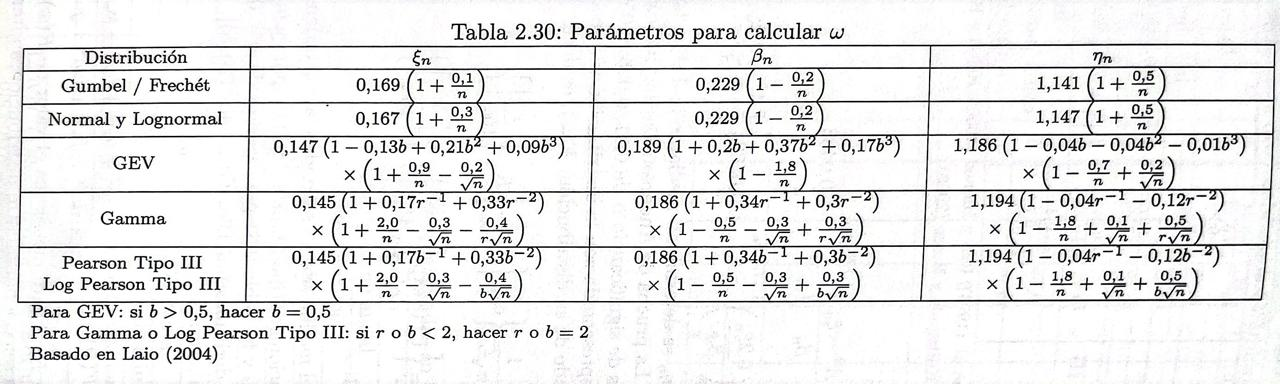
\includegraphics[width=1.0\linewidth]{taM230.jpeg}  % from Diaz-Gra
\end{frame}

\begin{frame}{Anderson-Darling test}
The \emph{Anderson-Darling test} shows that if $\omega < \omega_*$, where $\omega_* = 0.743, 0.581, 0.461 \text{ and} 0.347$ for significant levels of $\alpha = 0.01, 0.025, 0.05 \text{ and} 0.1$, $H_0$ is accepted, which means that the annual series can be represented by the chosen distribution. Alternatively, with the value of $\omega$, $F$ is calculated as as:
\[
    F(\omega) = \frac{1}{\pi \sqrt{\omega}} \left[ e^{\left(-\frac{1}{16\omega} \right)} K_{1/4}\left(\frac{1}{16\omega} \right) \right] + \frac{1}{\pi \sqrt{\omega}} \left[ 1.118 e^{\left(-\frac{25}{16\omega} \right)} K_{1/4} \left(\frac{25}{16\omega} \right) \right] \text{ for } \omega < 1.2 
        \]
        \[
            F(\omega) = 1 \text{ for } \omega \geq 1.2
        \]
        where $K_{1/4} [.]$ is the modified \emph{Bessel function} of order $1/4$. If $F(\omega) < (1-\alpha)$, $H_0$ is accepted; the lesser $F(\omega)$ the more suitable is the distribution chosen. 
\end{frame}

\begin{frame}{Distribution fitting}
  \begin{exampleblock}{Annual series of maximum streamflow at Banco station, Magdalena River} % from Diaz-Gra
\centering
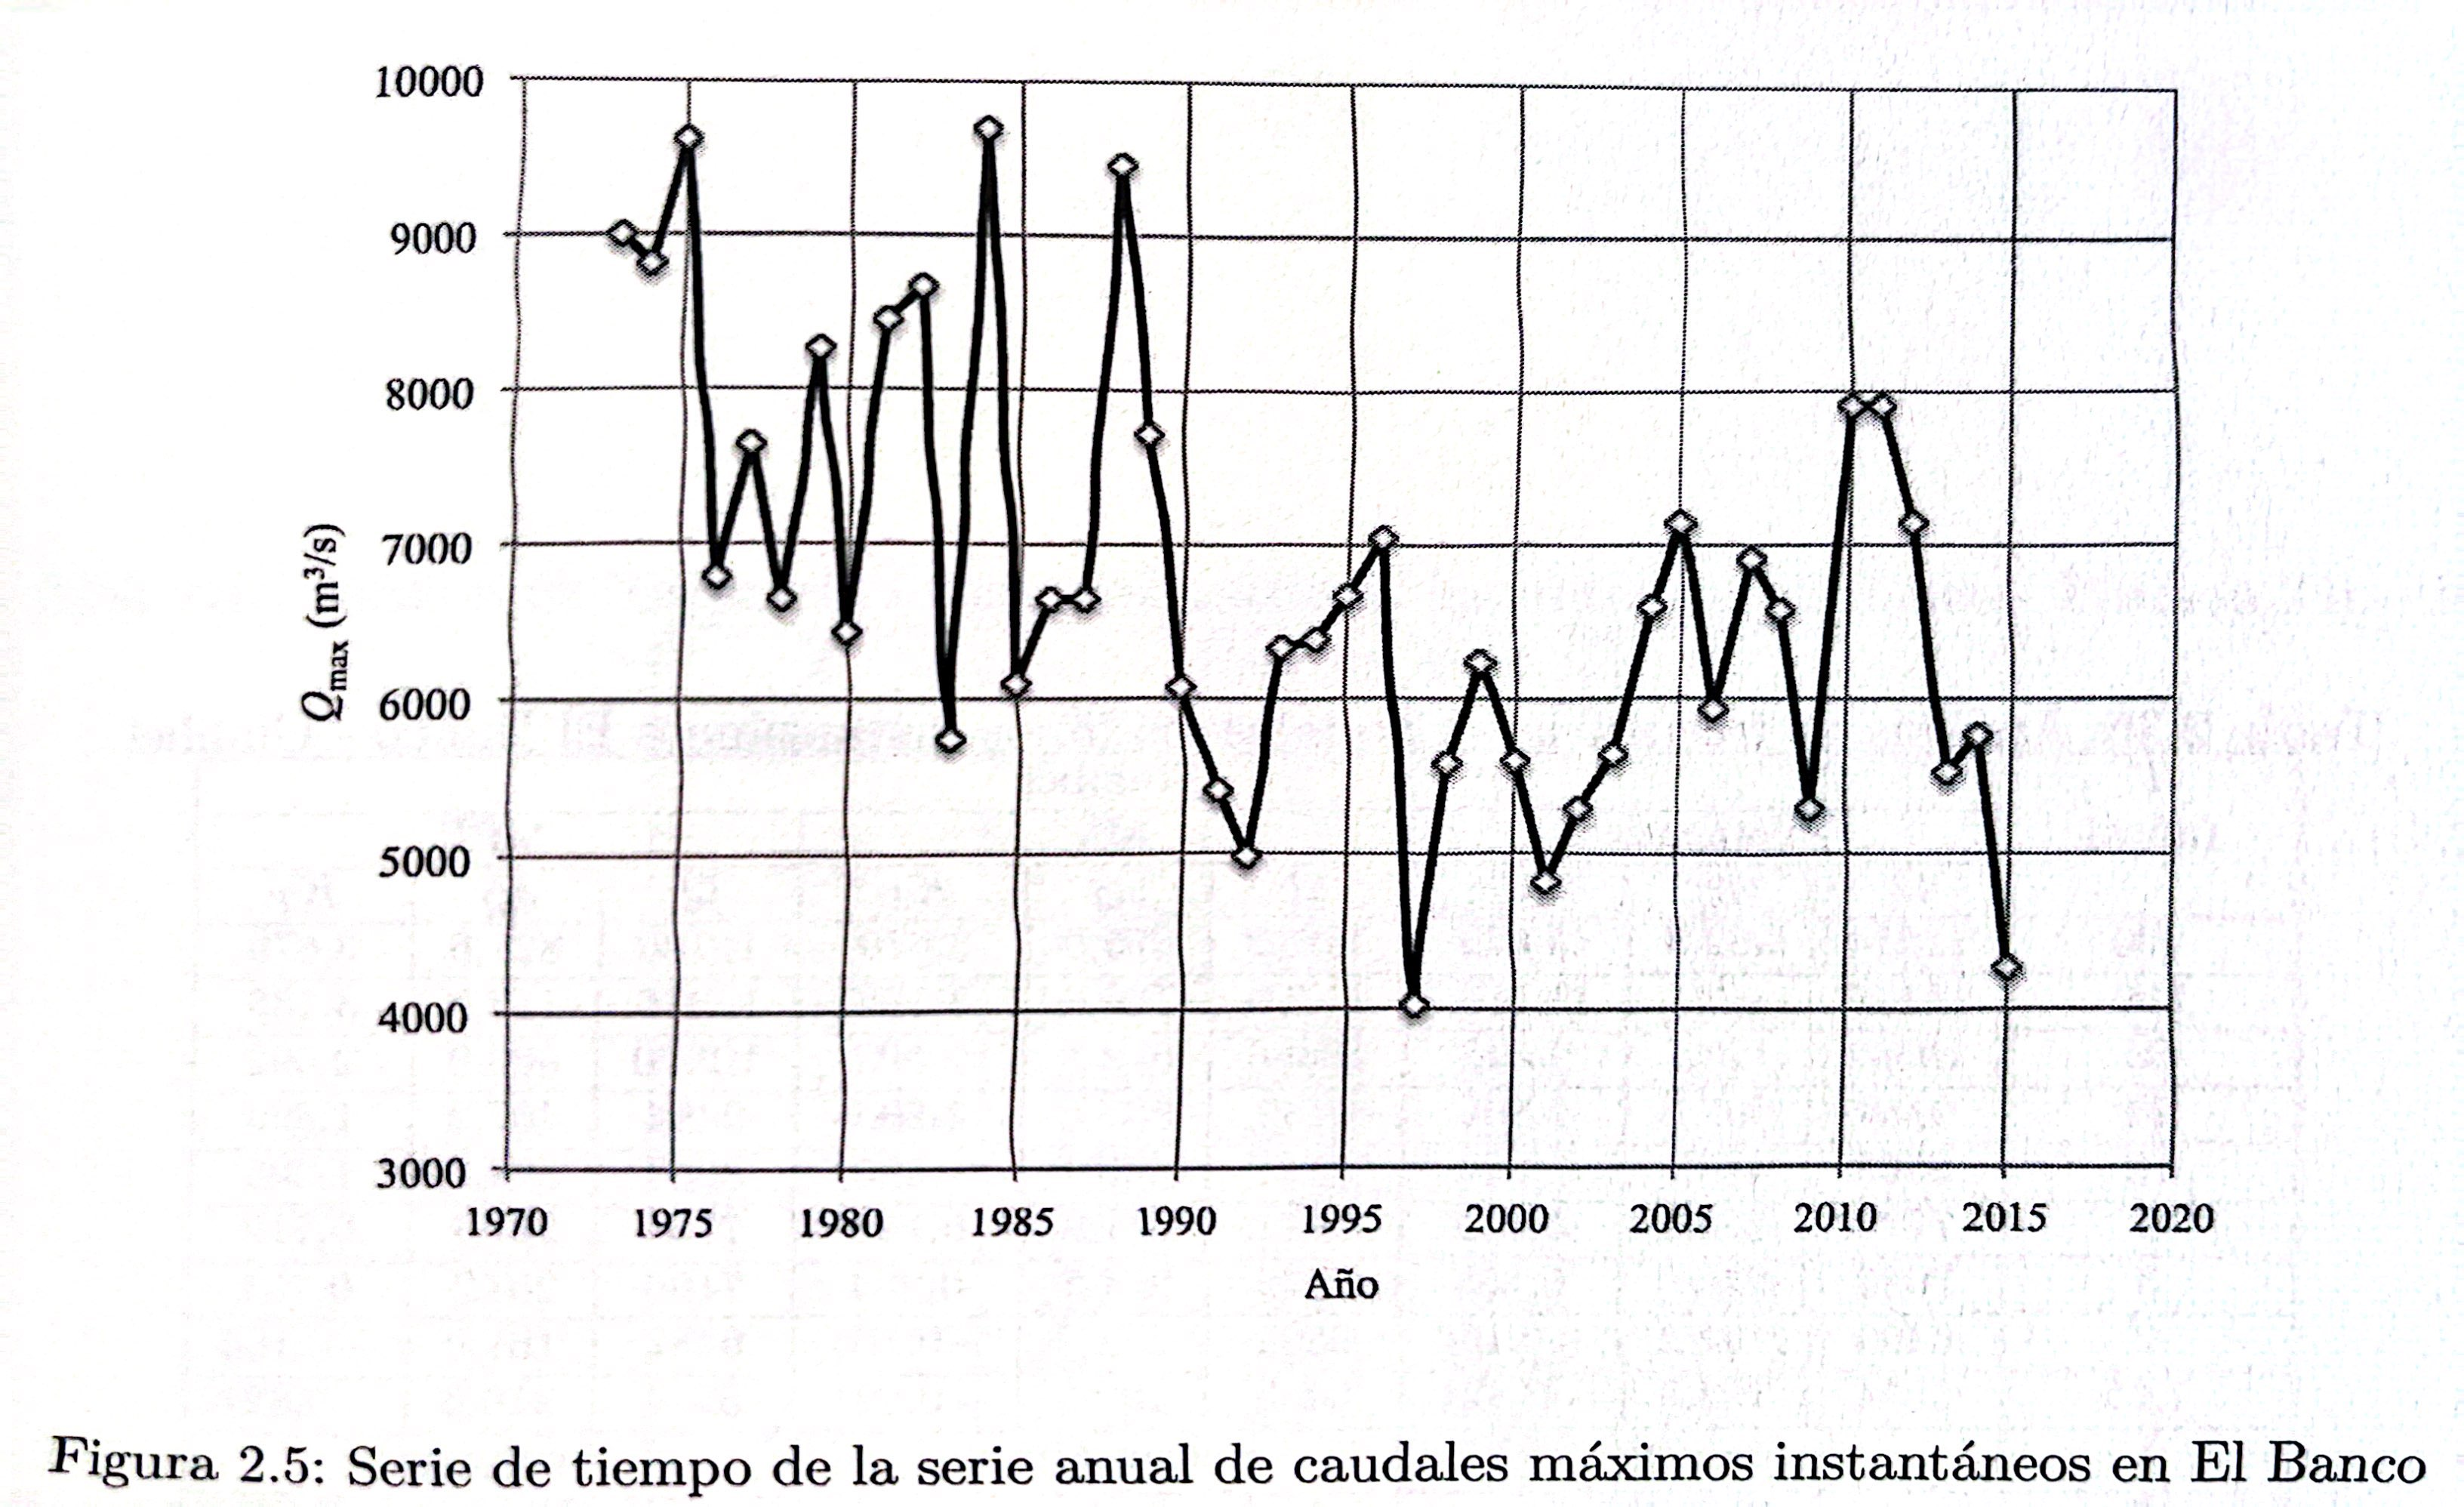
\includegraphics[width=1.0\linewidth]{fiM25.jpg}  % from Diaz-Gra
 \end{exampleblock}
\end{frame}

\begin{frame}{Distribution fitting}
  \begin{exampleblock}{Annual series of maximum streamflow at Banco station, Magdalena River} % from Diaz-Gra
\centering
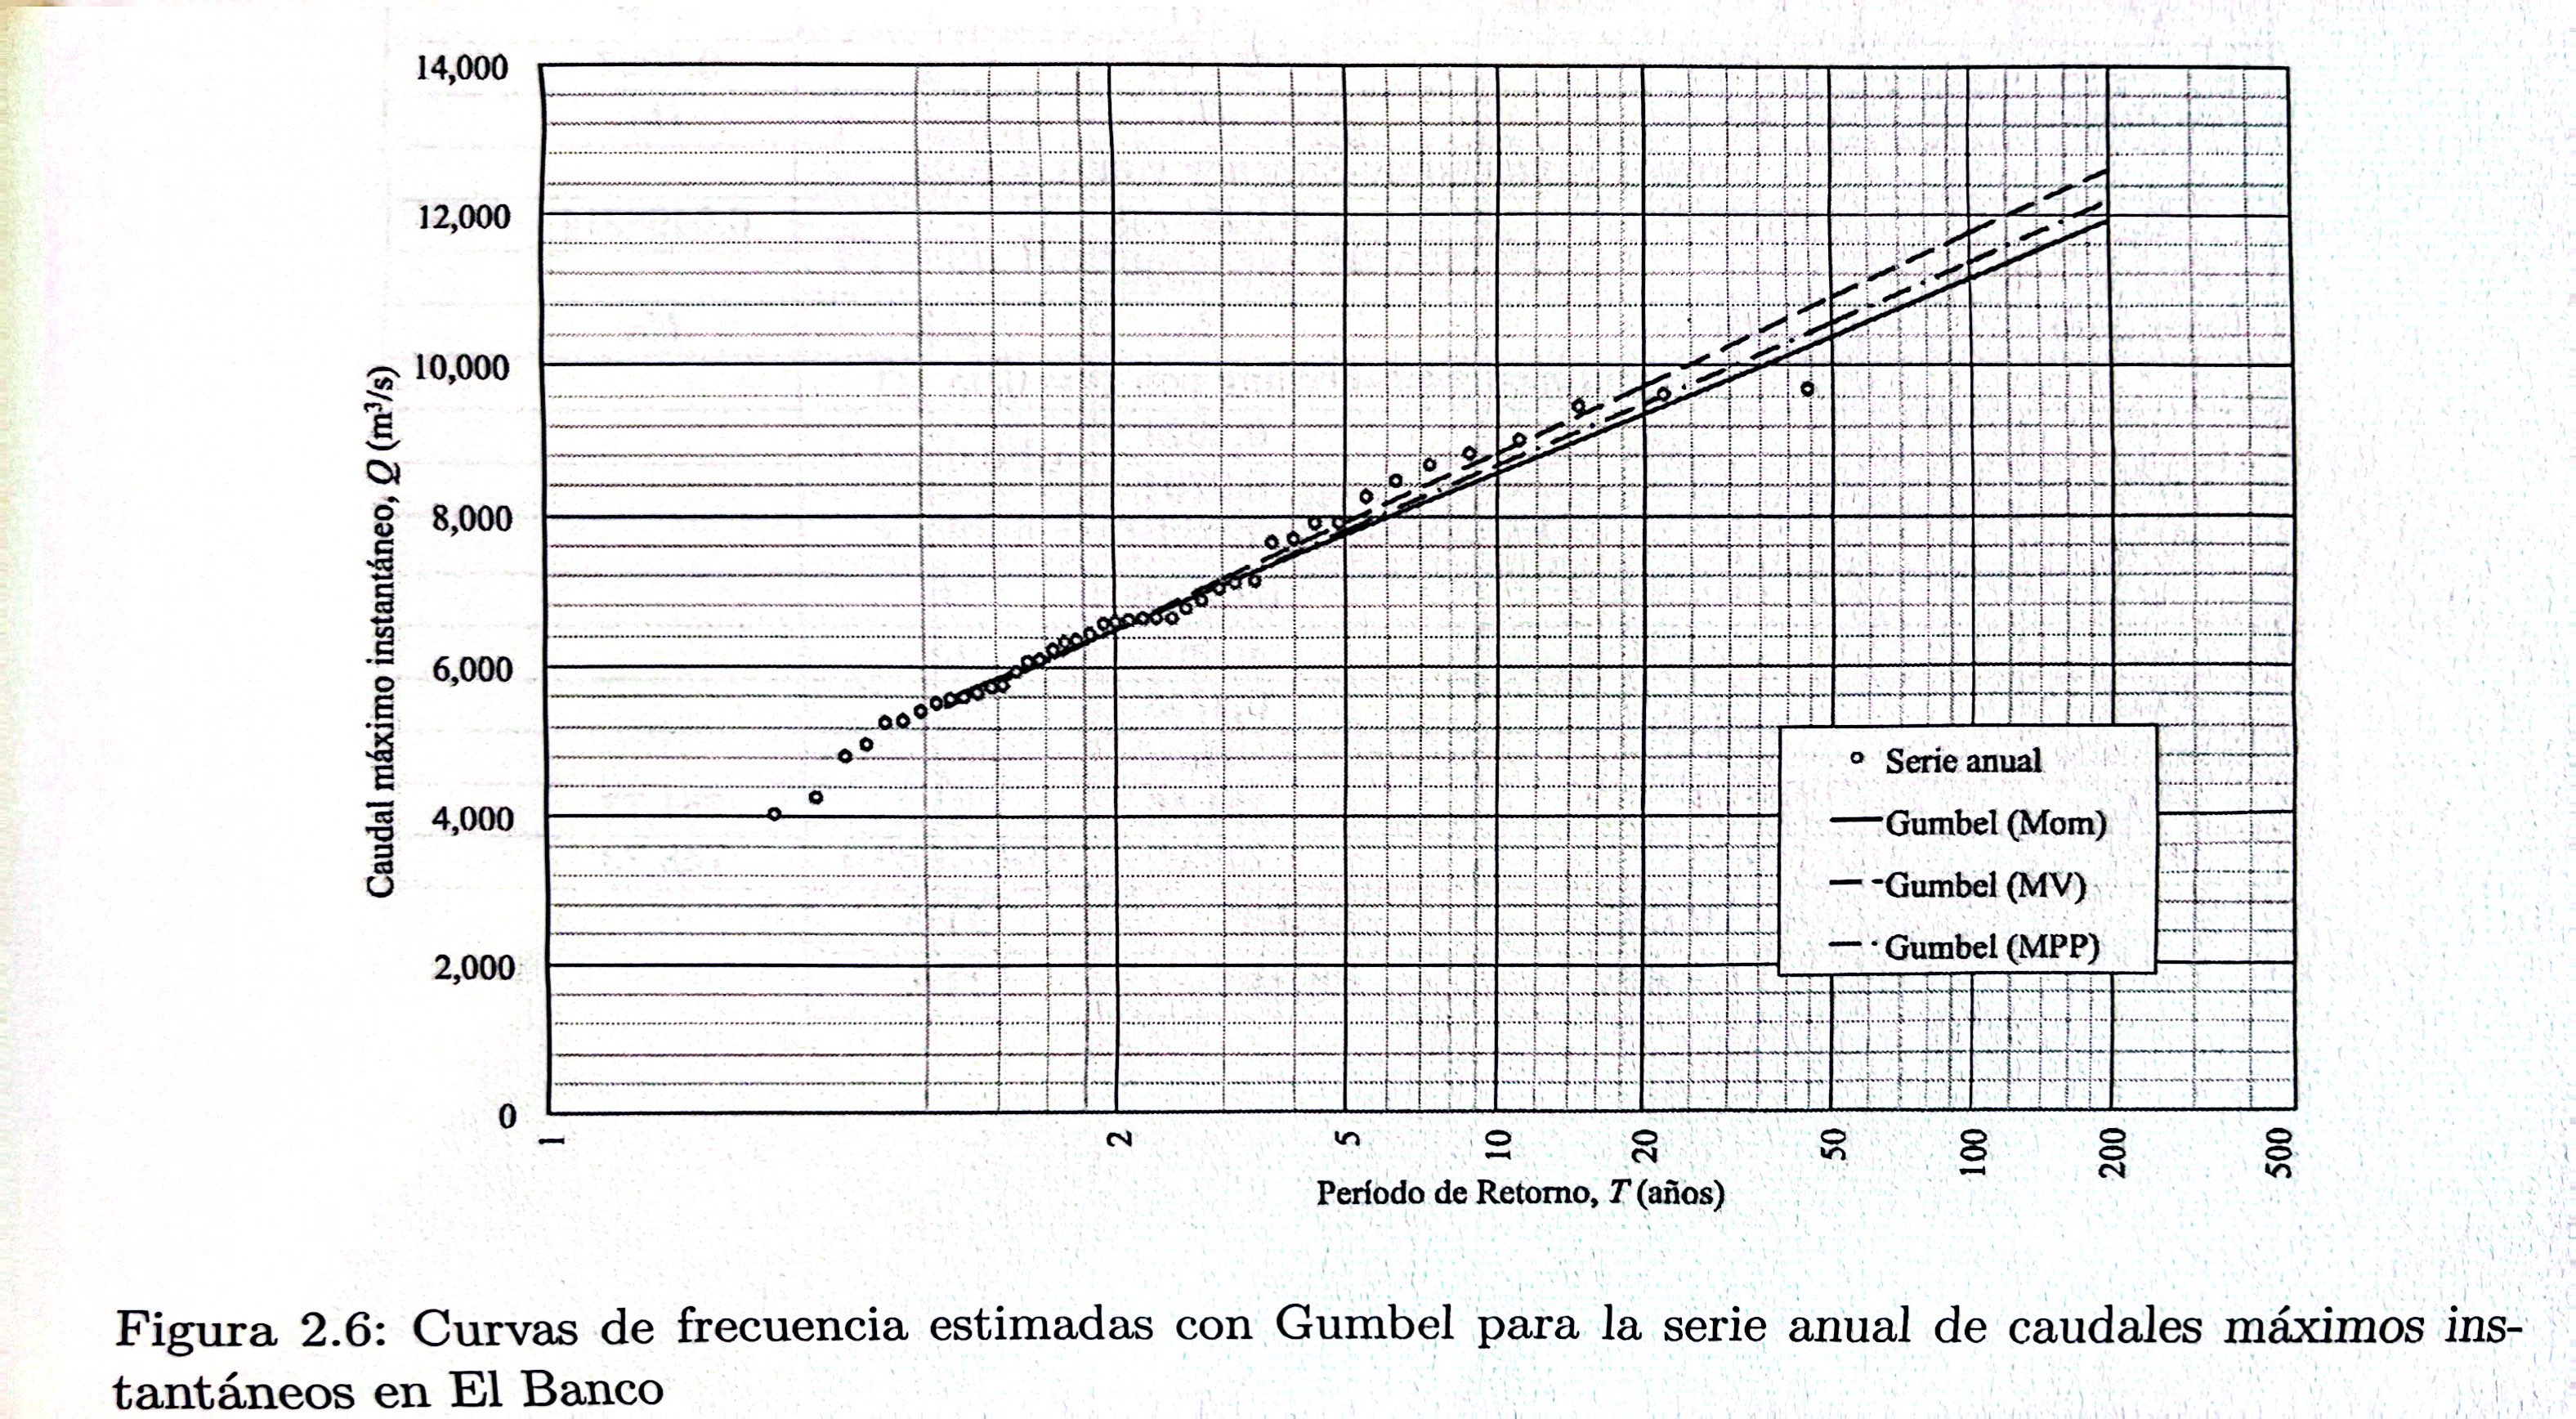
\includegraphics[width=1.0\linewidth]{fiM26.jpg}  % from Diaz-Gra
 \end{exampleblock}
\end{frame}

\begin{frame}{Distribution fitting}
  \begin{exampleblock}{Annual series of maximum streamflow at Banco station, Magdalena River} % from Diaz-Gra
\centering
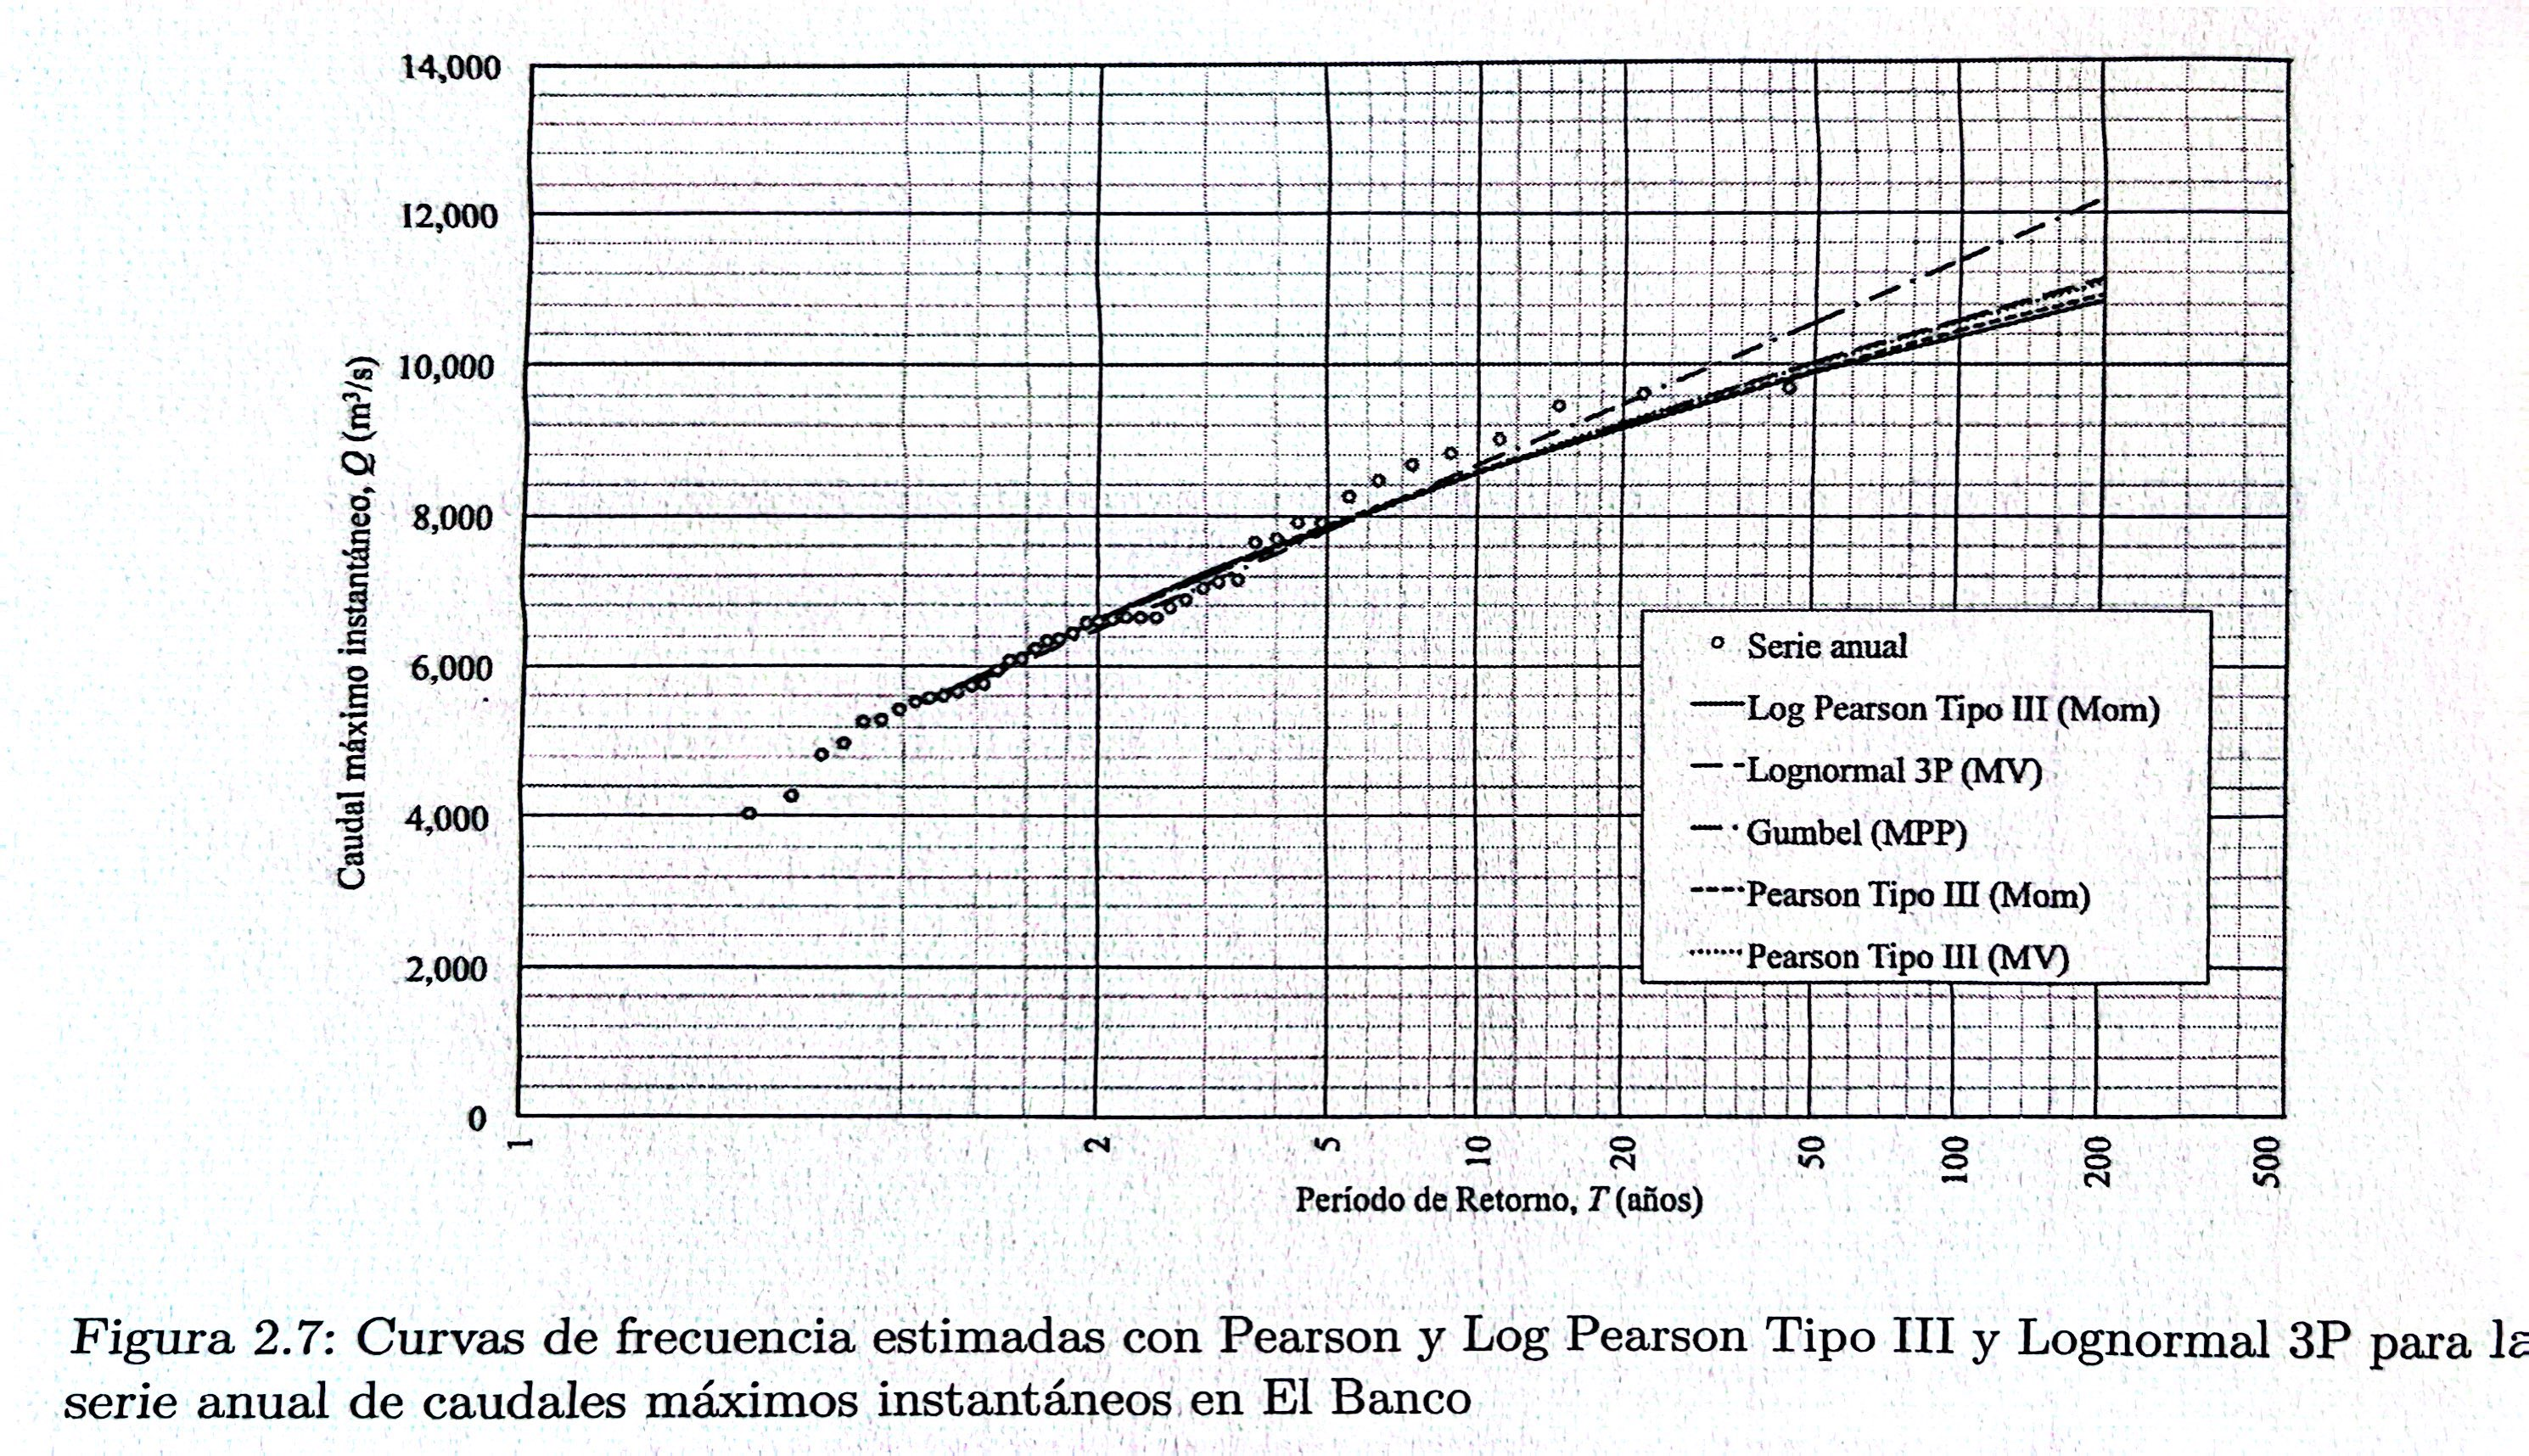
\includegraphics[width=1.0\linewidth]{fiM27.jpg}  % from Diaz-Gra
 \end{exampleblock}
\end{frame}

\begin{frame}{Distribution fitting}
  \begin{exampleblock}{Annual series of maximum streamflow at Banco station, Magdalena River} % from Diaz-Gra
\centering
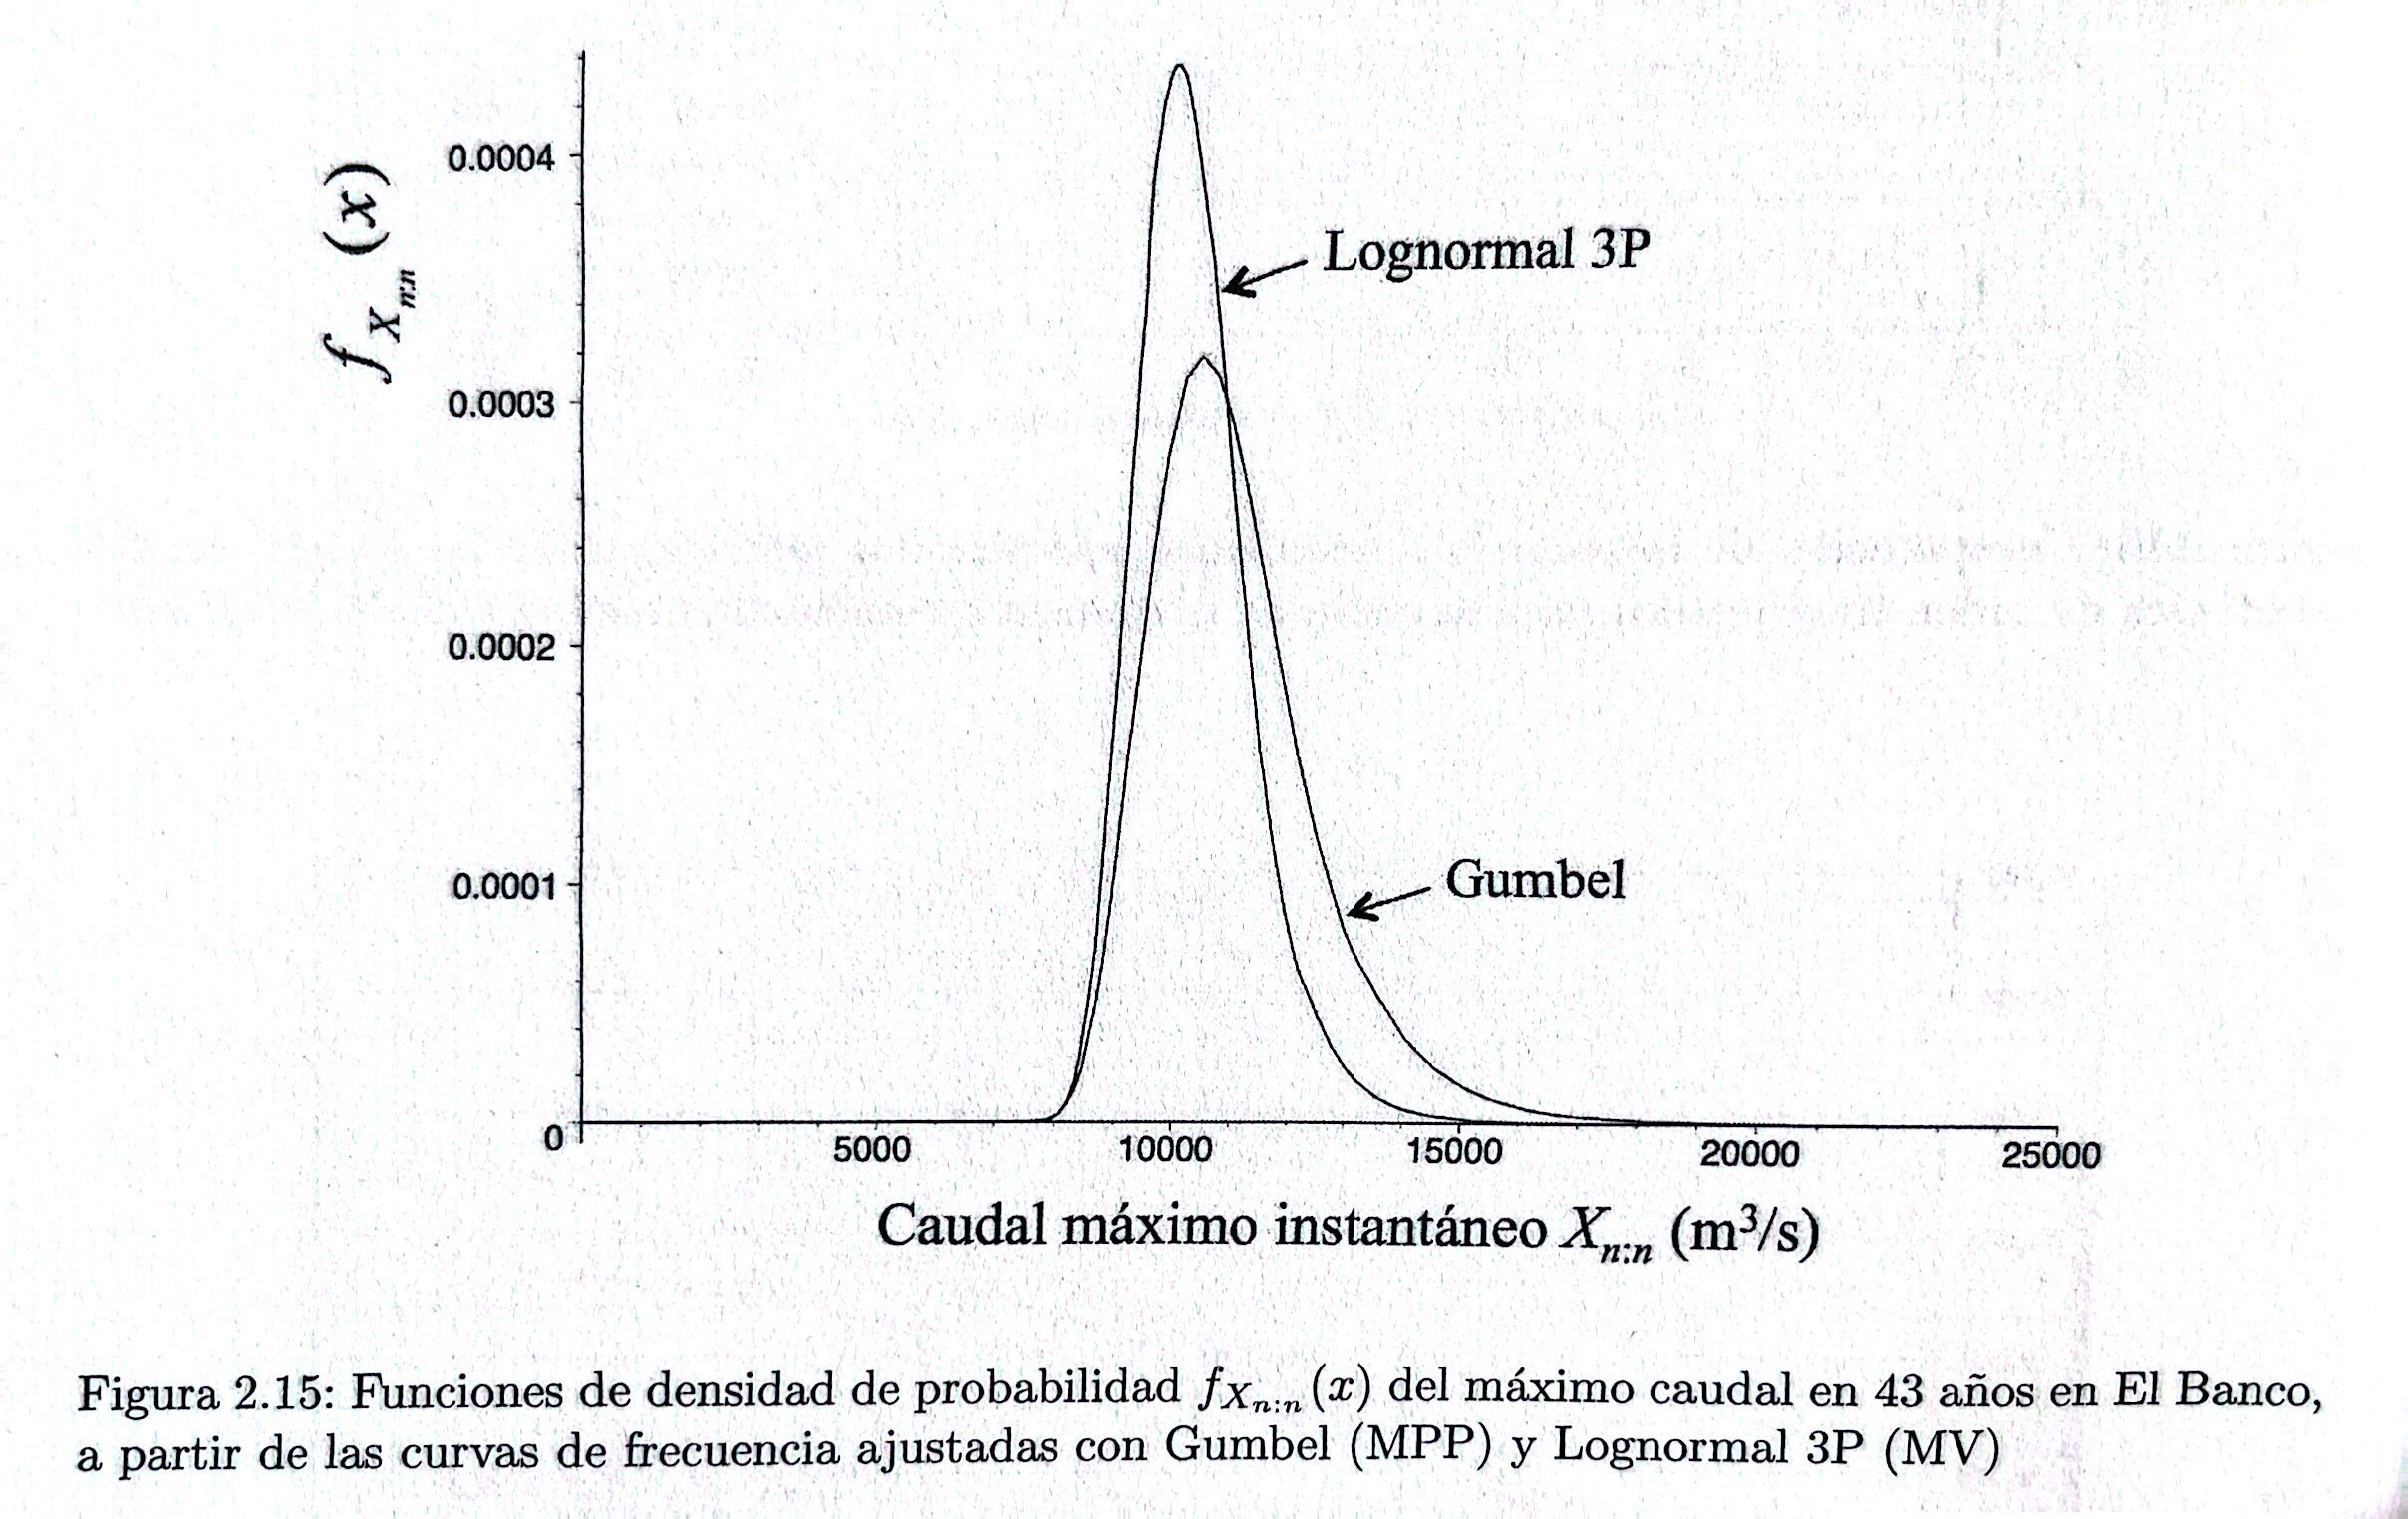
\includegraphics[width=1.0\linewidth]{fiM215.jpg}  % from Diaz-Gra
 \end{exampleblock}
\end{frame}


%-------
% From Diaz-granados
\section{Distribution selection}
\subsection{Generalities}
\begin{frame}{Generalities}
    The processes described above can be applied to any type of distribution using the different parameter-estimation methods. HERERE
\end{frame}





\end{document}

